\chapter{Leyes de la mecánica y el Problema de $N$ cuerpos}
\noindent
Cambiaremos ahora de problemas a estudiar, los cuales comienzan con la ley:
\begin{equation*}
    m\cdot a = F
\end{equation*}
Tenemos una partícula de la que queremos conocer su posición a lo largo del tiempo, $x(t)\in \mathbb{R}^d$, con $d\geq 1$ y a quien llamamos \textit{número de grados de libertad}. La masa $m$ será constante, la aceleración es $a = \ddot{x}(t)$ y la fuerza la consideramos $F = F(t,x,\dot{x})$. Así, la segunda Ley de Newton da lugar a la ecuación (o sistema de ecuaciones para $d>1$):
\begin{equation*}
    m\ddot{x} = F(t,x,\dot{x})
\end{equation*}

\begin{ejemplo}
    Vemos varios ejemplos:
    \begin{enumerate}
        \item Un primer ejemplo es la ecuación del muelle, podemos imaginar que tenemos una pared en $-\infty$ y que tenemos una masa $m$ atada a la pared con un muelle. Tenemos $d=1$ e imaginamos que el muelle comienza en una posición $x=0$ y que en el instante $t$ se encuentra en la posición $x(t)$.

            \begin{figure}[H]
                \centering
             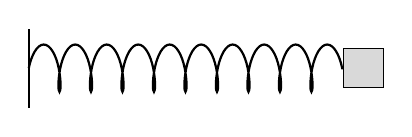
\begin{tikzpicture}
                % Dibuja la pared
                \draw[thick] (0,0.5) -- (0,1.5);

                % Dibuja el muelle
                \draw[thick, decoration={aspect=0.3, segment length=4mm, amplitude=3mm, coil}, decorate] (0,1) -- (4,1);

                % Dibuja el corcho como un cuadrado
                \draw[fill=gray!30] (4,0.75) rectangle (4.5,1.25);
            \end{tikzpicture}               
            \caption{Muelle atado a la pared.}
            \label{fig:muelle}
            \end{figure}

            \noindent
            Cuando $x(t) > 0$ tendremos que el muelle tira hacia la izquierda, por lo que $F(t,x(t),\dot{x}(t)) < 0$ y cuando $x(t) < 0$ tendremos que el muelle tira hacia la derecha, de donde $F(t,x(t),\dot{x}(t)) > 0$. Otra propiedad evidente es que la fuerza debe ser una función creciente en módulo en función de $x$. Así, típicamente se escoge el campo de fuerzas conocido como \textit{Ley\footnote{Aunque no describe el movimiento real de un muelle, es una aproximación.} de Hooke}:
            \begin{equation*}
                F(x) = -kx, \qquad k>0
            \end{equation*}
            Y a $k$ se le llama \textit{constente de elasticidad}, que mide ``lo duro que es el muelle''. Obtenemos aplicando la segunda Ley de Newton la ecuación del oscilador armónico:
            \begin{equation*}
                m\ddot{x} = -kx
            \end{equation*}
        \item En otra situación, imaginamos que tenemos un paracaidista, y que queremos conocer su altura sobre la superficie, $y(t)$. Pensaremos que $-\infty$ es estar muy lejos de la superficie.

            \begin{figure}[H]
                \centering
                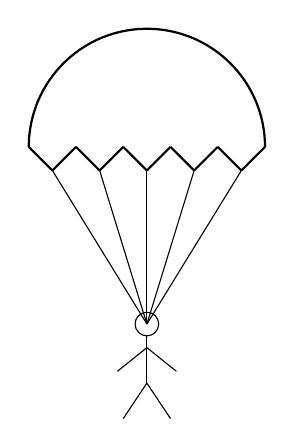
\begin{tikzpicture}[scale=0.75]

                % Parachute canopy (más pequeño)
                \draw[thick] (-2,0) arc (180:0:2);
                \draw[thick] (-2,0) -- (-1.6,-0.4);
                \draw[thick] (-1.6,-0.4) -- (-1.2,0);
                \draw[thick] (-1.2,0) -- (-0.8,-0.4);
                \draw[thick] (-0.8,-0.4) -- (-0.4,0);
                \draw[thick] (-0.4,0) -- (0,-0.4);
                \draw[thick] (0,-0.4) -- (0.4,0);
                \draw[thick] (0.4,0) -- (0.8,-0.4);
                \draw[thick] (0.8,-0.4) -- (1.2,0);
                \draw[thick] (1.2,0) -- (1.6,-0.4);
                \draw[thick] (1.6,-0.4) -- (2,0);

                % Suspension lines
                \draw (-1.6,-0.4) -- (0,-3);
                \draw (-0.8,-0.4) -- (0,-3);
                \draw (0,-0.4) -- (0,-3);
                \draw (0.8,-0.4) -- (0,-3);
                \draw (1.6,-0.4) -- (0,-3);

                % Skydiver
                \draw (0,-3) circle (0.2); % head
                \draw (0,-3.2) -- (0,-4); % body
                \draw (0,-3.4) -- (-0.5,-3.8); % left arm
                \draw (0,-3.4) -- (0.5,-3.8); % right arm
                \draw (0,-4) -- (-0.4,-4.6); % left leg
                \draw (0,-4) -- (0.4,-4.6); % right leg

                \end{tikzpicture}            
            \end{figure}
            \noindent
            Las fuerzas que están actuando sobre el paracaidista son:
            \begin{itemize}
                \item $F_1$, la fuerza del peso, que es constante:
                    \begin{equation*}
                        F_1 = mg
                    \end{equation*}
                \item $F_2$, la fueza de resistencia que hace el paracaidas, buscamos algo proporcional a la velocidad:
                    \begin{equation*}
                        F_2 = -k\dot{y}
                    \end{equation*}
                    Sin embargo, empíricamente se ve que ecuaciones lineales no son buenas para representar el rozamiento, por lo que lo consideraremos cuadrático:
                    \begin{equation*}
                        F_2 = -k|\dot{y}|\dot{y}
                    \end{equation*}
            \end{itemize}
            Obtenemos así finalmente la ecuación:
            \begin{equation*}
                m\ddot{y} = mg - k|\dot{y}|\dot{y}
            \end{equation*}
            Y sabemos que hay existencia y unicidad (puesto que es de clase 1).
        \item El siguiente ejemplo es el más relevante y el que hizo nacer la teoría de las ecuaciones diferenciales, el \textbf{Problema de los 2 cuerpos}.

            Tenemos dos planetas, uno de masa $m_1$ y otro más chico de masa $m_2$. Supondremos siempre que son dos puntos de masas, no volúmenes. Cada planeta tiene asociada su posición en el espacio, $p_1,p_2:\mathbb{R}\to \mathbb{R}^3$.

            En el planeta de masa $m_1$ tenemos la fuerza gravitatoria que ejerce el planeta 2 sobre el 1, $F_{21}$, y en el planeta de masa $m_2$ tenemos la fuerza que ejerce el planeta 1 sobre el 2, $F_{12}$.

            \begin{figure}[H]
                \centering
                \begin{tikzpicture}[scale=1]

                % Mass m1 (más grande)
                \draw[fill=gray!30] (0,0) circle (0.8);
                \node at (0,0) {$m_1$};

                % Mass m2 (más pequeña)
                \draw[fill=gray!30] (5,0) circle (0.4);
                \node at (5,0) {$m_2$};

                % Fuerza sobre m1 debida a m2
                \draw[-Stealth, thick] (0.8,0) -- (2.3,0);
                \node[above] at (1.55,0) {$F_{21}$};

                % Fuerza sobre m2 debida a m1
                \draw[-Stealth, thick] (4.6,0) -- (3.1,0);
                \node[above] at (3.85,0) {$F_{12}$};

                \end{tikzpicture}
            \end{figure}

            \noindent
            Los físicos nos dicen que (en mecánica siempre se considera la norma euclídea):
            \begin{align*}
                F_{21} &= \frac{Gm_1m_2}{\|p_1-p_2\|^2} \frac{p_2-p_1}{\|p_2-p_1\|} \\
                F_{12} &= -F_{21}
            \end{align*}
            La ecuación del movimiento en un universo que solo tuviera dos masas queda como:
            \begin{equation*}
                \left\{\begin{array}{l}
                    m_1\ddot{p_1} = \dfrac{Gm_1m_2}{\|p_1-p_2\|^3}(p_2-p_1) \\
                    \\
                    m_2\ddot{p_2} = \dfrac{Gm_1m_2}{\|p_1-p_2\|^3}(p_1-p_2)
                \end{array}\right.
            \end{equation*}
            Y como tenemos $p_i = (x_i, y_i, z_i)$ para $i \in \{1,2\}$, tenemos 6 grados de libertad. La primera ecuación de ellas sería:
            \begin{equation*}
                m_1\ddot{x}_1 = \frac{Gm_1m_2}{\left[{(x_1-x_2)}^{2} + {(y_1-y_2)}^{2} + {(z_1-z_2)}^{2}\right]^{\nicefrac{3}{2}}} (x_2-x_1)
            \end{equation*}
        \item Consideramos ahora para $N>2$ el Problema de $N$ cuerpos.

            Tenemos ahora 3 masas, $m_1,m_2,m_3$ y sobre cada una de ellas actúan $N-1$ fuerzas:
            \begin{equation*}
                m_i \ddot{p}_i = \sum_{j\neq i} \frac{Gm_im_j}{\|p_i-p_j\|^3}(p_j-p_i), \qquad i = 1, \ldots,N
            \end{equation*}
            Aquí tenemos $x=(p_1,\ldots,p_N)\in \mathbb{R}^{3N}$, al que llammos \textit{espacio de configuraciones}.
            Para tratar de resolver el sistema, tomamos $v_i = \dot{p}_i$ y pasamos a:
            \begin{equation*}
                \left\{\begin{array}{l}
                        \\
                        \dot{p}_i = v_i \\
                        \\
                        \dot{v}_i = \displaystyle \sum_{j\neq i} \frac{Gm_j}{\|p_i-p_j\|^3}(p_j- p_i)
                \end{array}\right.
            \end{equation*}
            Y tenemos $x = (p_1, \ldots, p_N, v_1, \ldots, v_N)\in \mathbb{R}^{6N}$, al que llamamos \textit{espacio de fases}.
    \end{enumerate}
\end{ejemplo}


